\documentclass[12pt]{article}
\renewcommand{\baselinestretch}{1.5}
%%%%%%%%%%packages
\usepackage[english]{babel}
%%%%%%%%%%%%%%%%%%%%%%%%%%%%%%%%%%%%%%%%%
%%%%%%%%%%%%%%%%%%%%%%%%%%%%%%%%%%%%%%%%
\usepackage[latin1]{inputenc}
%%%%%%%%%%%%%%%%%%%%%%%%%%%%%%%%%%%%%%%%
%%%%%%%%%%%%%%%%%%%%%%%%%%%%%%%%%%%%%%%%%
\PassOptionsToPackage{usenames,dvipsnames}{xcolor}
\usepackage[dvips]{graphicx,psfrag,overpic,color} %Necesario para figuras
\usepackage{latexsym} %Necesario para simbolos ampliados
\usepackage{amssymb} %Necesario para simbolos AMS
\usepackage{amsmath}%Necesario para simbolos AMS extra
\usepackage{amsfonts}%Necesario para fuentes AMS extra
\usepackage{amsthm}
\usepackage{pstricks}  % since the dash is rendered by pstricks!
\usepackage[postscript]{ucs}
\usepackage{fancyhdr}
\usepackage{listings}
\usepackage[a4paper,left=3cm,right=3cm,top=2.5cm,bottom=2.5cm]{geometry}
\usepackage{url}
\usepackage{pdfpages}
\usepackage{mathtools}
\usepackage{titling}
\usepackage[nottoc,numbib]{tocbibind}
\usepackage{mathptmx}
\usepackage[explicit]{titlesec}
\usepackage{pgfplots}
\usepackage{float}

\titleformat{\section}[block]{\filcenter}{\thesection. \MakeUppercase{#1}}{1em}{}
\titleformat{name=\section, numberless}[block]{\filcenter}{\MakeUppercase{#1}}{1em}{}
\titleformat{\subsection}[hang]{}{}{1em}{\thesubsection. #1}
\titleformat{\subsubsection}[hang]{}{}{1em}{{\normalfont\thesubsubsection. \textit{#1}}}


\newtheorem{theorem}{{Theorem}}
\newtheorem{prop}{{Proposition}}
\newtheorem{defi}{{Definition}}
\newtheorem{claim}{{Claim}}

\makeindex

\pretitle{%
  \begin{center}
  \LARGE
  \vspace{1in}
  
\includegraphics[width=4.56in]{logo_uab2}\\[\bigskipamount]
  \vspace{1.5in}
}
\posttitle{\end{center}}

\begin{document}


\selectlanguage{english}

\title{{\large TITLE: Merger Simulations: A Theoretical and Practical Approach\\
AUTHOR: Andrea Dana Klein Villalba\\
DEGREE: Economics\\
ADVISOR: Jordi Perdiguero Garc\'ia\\
DATE: June 7th, 2019\\}}
\date{}

%-------------------------------------------------------------%
\clearpage\maketitle
\thispagestyle{empty}
\newpage

\begin{abstract}
Hello, it's me,
\end{abstract}
\newpage

%--------------------------------------------------------------
% Taula de continguts
% S'elabora automaticament
%-------------------------------------------------------------
 \tableofcontents
 \newpage
%------------------------------------------------------------
% Cos del treball
%Es poden fer servir Parts, Capitols, Seccions i Subseccions
%-------------------------------------------------------------
\pagenumbering{arabic}

\section{Introduction}

When we are first introduced into economic theory, we start talking about perfect competition models, where a single supplier's or consumer's decision does not affect the market. However, these models are far from the truth, which raises the question about how market power affects market equilibria.\\
This has been the conundrum that researchers and policy makers have faced and continue to do so. Theoretically, in the presence of market concentration, firms tend to perceive a higher level of profits, while consumer welfare is reduced. When we translate this theory into the real world, we find that most markets have some concentration of market power, and so we try to measure the impact that changes -or mergers- may have in it. Since this technique relies on quantitative estimations of demand and cost functions, there is some skepticism around it (\cite{peters} Peters, 2006). But even though it may be somewhat limited by the models, researchers do recognize its usefulness. Other researchers focus on the use of merger simulation and its implementation, particularly for antitrust and competition agencies, (\cite{ivaldi} \cite{bjorn} Ivaldi and Verboven, 2005; Bj\"{o}rnerstedt and Verboven, 2015), finding that the models do make correct predictions to an extent. \\
Another common issue is actually computing the mergers. When teaching oligopolies and mergers, we focus on markets where initially there are two producers, since that leads to relatively simple equations. These allow us to get an intuitive idea about what would happen in a market with three players, and so forth. However, when we want to analyze a market with more than two players, we find that our equations become considerably complex. This is where computer science comes into play, introducing programming into economic theory. This idea is far from new, and Davis (2006) \cite{davis} already defined a theoretical approach to compute mergers with linear demands and constant marginal costs.\\
Thus, in this project, we continue on Davis's (2006) \cite{davis} and we seek to create a tool that enables researchers, teaching staff, and students to easily compute and better understand the effects of a merger in a market with different characteristics. Hence, this project may contribute to better and more precise assessments of competition and market regulation.\\
Therefore, we propose a program that does so for several combinations of demands and costs, with pure algebraic methods and numerical methods when the former is not possible. In this project we will describe the different models to be used, then move on to give user instructions, and move forward by proposing future applications and developments. 


\section{Models}

The models used in this project are characterized by Bertrand Competition, where the suppliers choose prices according to demand. This will be modeled as an economy in which there are $N$ products and $M$ different firms that produce them.

\begin{defi}
The set of products is denoted by $\mathcal{N} = \{1, 2, \dots, N\}$ and the subset of products produced by the same firm will be written as $\mathcal{N}_m \subseteq \mathcal{N}$. The set of firms will be written as $\mathcal{M}$.
\end{defi}

It is important to note that each product is exactly produced by one firm, i.e.  $\mathcal{N}_{m_1} \cap \mathcal{N}_{m_2} = \emptyset$ if $m_1$ and $m_2$ are two different firms and $\bigcup\limits_{m\in\mathcal{M}} \mathcal{N}_m = \mathcal{N}$. The firms in this economy will be profit-maximizing firms, and therefore we can write their profit function as
\begin{equation}
\pi_m(p) = \sum_{j \in \mathcal{N}_m} (p_j - c_j) \cdot q_j(p) \label{profit_eq}
\end{equation}

Where $p = (p_1, p_2, \dots, p_N)^t$ is the column vector of prices, and $c_j = \frac{\partial C_j}{\partial q_j}$ are the marginal costs and $q_j$ is the demand for the $j$-th good. 

\begin{defi}
The demand function $q$ is
\begin{eqnarray*}
q: ~ \mathbb{R}^N & \rightarrow & \mathbb{R}^N \\
p & \mapsto & q(p)
\end{eqnarray*}
where $q(p) = (q_1(p), q_2(p), \dots, q_N(p))^t$ is the column vector of the demands.
\end{defi}

\begin{defi}
The marginal cost function $c$ is
\begin{eqnarray*}
c: ~ \mathbb{R}^N & \rightarrow & \mathbb{R}^N \\
q & \mapsto & c(q)
\end{eqnarray*}
where $c(q) = (c_1(q_1), c_2(q_2), \dots, c_N(q_N))^t$ is the column vector of the marginal costs.
\end{defi}

Notice that, while $c(q)$ is a function of $q$, the latter is also a function of $p$, so $c(q)$ is a function of $p$ as well. 

For the given profit function, it is maximized when the first order conditions are fulfilled. Such that, deriving from equation \ref{profit_eq} with respect to $p_k$ such that $k \in \mathcal{N}_m$.
\begin{eqnarray}
\frac{\partial \pi_m}{\partial p_k} &=& \frac{\partial}{\partial p_k} \sum_{j \in \mathcal{N}_m} (p_j - c_j(q_j)) \cdot q_j(p) \\
&=& \sum_{j \in \mathcal{N}_m} \frac{\partial}{\partial p_k} \left[(p_j - c_j(q_j)) \cdot q_j(p)\right] \\
&=& \sum_{j \in \mathcal{N}_m} q_j(p) \frac{\partial (p_j - c_j)}{\partial p_k}(q_j) + \sum_{j \in \mathcal{N}_m} \frac{\partial q_j}{\partial p_k}(p) \cdot (p_j - c_j(q_j))\\
&=& q_k(p) - \sum_{j \in \mathcal{N}_m} q_j(p) \frac{\partial c_j}{\partial p_k} (q_j) + \sum_{j \in \mathcal{N}_m} \frac{\partial q_j}{\partial p_k}(p) \cdot (p_j - c_j(q_j)) = 0 \label{profit_FOC_eq}
\end{eqnarray}

Since each product is produced by exactly one firm, deriving as so for each product, we obtain a system of $N$ equations that is solved for the optimal prices $p^*$. In order to solve this system, it is useful to introduce the following variables:
\begin{defi}
Let $D = (d_{ij})$ be the ownership matrix of size $N \times N$, such that\\
\begin{center}
$d_{ij} = \left\{
\begin{tabular}{ll}
1 & if $i,j$ produced by the same firm\\
0 & otherwise
\end{tabular}\right.$
\end{center}
\end{defi}

By using the ownership matrix $D$, we can rewrite the first order condition from equation \ref{profit_FOC_eq} as follows
\begin{equation}
q_k(p) - \sum_{j=1}^N q_j(p) \frac{\partial c_j}{\partial p_k} (q_j)d_{jk} + \sum_{j=1}^N \frac{\partial q_j}{\partial p_k}(p) \cdot (p_j - c_j(q_j))d_{jk} = 0 \label{profit_FOC_with_Ds_eq}
\end{equation}

Finally, we need a measure of welfare. For the producer welfare (or surplus), we compute the profits for the prices $p^*$ and quantities $q^*$ at equilibrium. The consumer welfare $CW$, will be computed as follows
\begin{equation}
CW = \int_{p^*}^{p(q=0)} q(p) \ dp = \int_0^{q^*} p(q) \ dq \label{consumer_welfare_eq}
\end{equation}

\subsection{Linear Demands with Constant Marginal Costs}

In this model we will assume that demands are linear, such that
\begin{equation*}
q_k(p) = a_k + \sum_{j=1}^N b_{kj}p_j
\end{equation*}

Because marginal costs are constant, the costs function $C_j$ will be characterized by
\begin{equation*}
C_j (q_j)= f_j + v_j \cdot q_j
\end{equation*}

Where $f_j$ is measure of fixed costs, $v_j$ is a measure of variable costs, and  $j \in \mathcal{N}$. Thus, marginal costs are
\begin{equation*}
c_j = \frac{\partial C_j}{\partial q_j}(q_j) = v_j
\end{equation*}

Computing the first order conditions from equation \ref{profit_FOC_with_Ds_eq}, we obtain
\begin{eqnarray*}
\frac{\partial\pi_m(p)}{\partial p_k}
&=& q_k(p) + \sum_{j = 1}^N d_{jk}b_{jk} \cdot (p_j - c_j) = 0
\end{eqnarray*}

Because we have one such first order condition for each product, we can write the system in a more compact way using matrices and vectors.
\begin{equation*}
a + B^t p + (D \circ B)(p - c) = 0
\end{equation*}

Where $\circ$ denotes the Hadamard product.
Isolating $p$, we obtain the optimum prices $p^*$
\begin{equation*}
p^* = (B^t + (D \circ B))^{-1}((D \circ B) c - a)
\end{equation*}

Then, optimum quantities are defined by
\begin{equation*}
q^* = a + B^t \cdot p^*
\end{equation*}

We are now interested in computing consumer welfare $CW$, following the form in equation \ref{consumer_welfare_eq}. 
\begin{equation*}
CW = \int_{p^*}^{p(q = 0)} q(p) dq = \frac{-q^*}{b_{kk}} \cdot q^*
\end{equation*}

\subsection{Linear Demands with Linear Marginal Costs}

In this model we will assume that demands are linear, such that
\begin{equation*}
q_k(p) = a_k + \sum_{j=1}^N b_{kj}p_j
\end{equation*}

Because marginal costs are linear, the costs function $C_j$ will be characterized by
\begin{equation*}
C_j(q_j) = f_j + v_j \cdot q_j + w_j \cdot q_j^2
\end{equation*}

Where $f_j$ is a measure of fixed costs, $v_j$ is a measure of linear variable costs, $w_j$ is a measure of quadratic variable costs, and $j \in \mathcal{N}$ Thus, marginal costs are
\begin{equation*}
c_j = \frac{\partial C(q_j)}{\partial q_j}= v_j + w_j \cdot q_j.
\end{equation*}

Computing the first order conditions from equatio \ref{profit_FOC_with_Ds_eq}, we obtain
\begin{equation*}
\frac{\partial\pi_m(p)}{\partial p_k} = q_k(p) + \sum_{j = 1}^N b_{jk} \cdot d_{jk} \cdot p_j - \sum_{j = 1}^N b_{jk} \cdot d_{jk} \cdot v_j - 2 \cdot \sum_{j = 1}^N b_{jk} \cdot d_{jk} \cdot w_j \cdot q_j (p) = 0
\end{equation*}

Because we have one such first order condition for each product, we can write the system in a more compact way using matrices and vectors. 
\begin{equation*}
a + B ^ t p + (D \circ B)(p - v - 2 \cdot w \cdot (a + B^t p)) = 0
\end{equation*}

Isolating $p$, we obtain the optimum prices $p^*$
\begin{equation*}
p^* = [B^t + (D \circ B) - 2 (D \circ B)(w \circ B^t]^{-1} \cdot [-a + (D \circ B) v + 2 (D \circ B)(w \circ a)]
\end{equation*}

Then, the optimum quantites are defined by
\begin{equation*}
q^* = a + B^t \cdot p^*
\end{equation*}

We are now interested in computing consumer welfare $CW$, following the form in equation \ref{consumer_welfare_eq}.
\begin{equation*}
CW = \int_{p^*}^{p(q = 0)} q(p) dq = \frac{-q^*}{b_{kk}} \cdot q^*
\end{equation*}

\subsection{Quadratic Demands with Constant Marginal Costs}

In this model we will assume that demands are quadratic, such that
\begin{equation*}
q_k(p) = a_k + \sum_{j=1}^N b_{kj}p_j + \sum_{j=1}^N e_{kj} p_j^2
\end{equation*}


Because marginal costs are constant, $C_j$ will be characterized by 
\begin{equation*}
C_j(q_j) = f_j + vj \cdot q_j
\end{equation*}

Where $f_j$ is a measure of fixed costs, $v_j$ is a measure of variable costs, and $j \in \mathcal{N}$. Thus, marginal costs are,
\begin{equation*}
c_j = \frac{\partial C_j(q_j)}{\partial q_j} = v_j
\end{equation*}

Computing the first order conditions from equation \ref{profit_FOC_with_Ds_eq}, we obtain
\begin{equation*}
\frac{\partial \pi_m(p)}{\partial p_k} = q_j(p) + \sum_{j=1}^N (d_{jk} \cdot b_{jk} + 2 \cdot d_{jk} \cdot e_{jk} \cdot p_k) \cdot (p_j - c_j) = 0
\end{equation*}

Because we have one such first order condition for each product, we can write the system in a more compact way using matrices and vectors.
\begin{equation*}
a +(B \circ D) p + (E \circ D) (p \circ p) + ((B \circ D) + 2 (E \circ D) p) (p - c) = 0 
\end{equation*}

Because this equation cannot be isolated for $p$, we obtain the optimum prices through the Newton-Raphson Method.

\begin{equation*}
P_{n+1} = P_n - J^{-1} \cdot F(P_n)
\end{equation*}

Where $J^{-1}$ is the inverse of the Jacobian matrix, and $F_j(P_n) = \partial \pi_m / \partial p_k$. The Jacobian matrix is constructed as follows

\begin{equation}
J_{ij} = \frac{\partial F_i}{\partial p_j} = \frac{\partial q_i(p)}{\partial p_j} + \sum_{j \in \mathcal{N}_m} \frac{\partial^2 q_i(p)}{\partial p_i \partial p_j} + \sum_{j \in \mathcal{N}_m} \frac{\partial q_i(p)}{\partial p_j}
\end{equation}

Then, the optimum quantities are defined by 
\begin{equation*}
q^* = a + B^t p^* + E^t p^{*2}
\end{equation*}

We are now interested in computing consumer welfare $CW_i$ following the form in equation \ref{consumer_welfare_eq}.
\begin{equation*}
CW_k = \int_0^{q_k^*} p_k(q_k) \ dq_k = -\frac{b_{kk}}{2 \cdot e_{kk}} \cdot q^* -\frac{1}{2 \cdot e_{kk}} \cdot \bigg[\frac{2}{12 \cdot e_{kk}} (b_{kk}^2 - 4 \cdot e_{kk}(H - q))^{\frac{3}{2}}\bigg]_0^{q^*} - p_k^* \cdot q_k^*
\end{equation*}

See appendix 1 for the computation of the integral in this model.  

\subsection{Quadratic Demands with Linear Marginal Costs}

In this model we will assume that demands are quadratic, such that
\begin{equation*}
q_k(p) = a_k + \sum_{j = 1}^N b_{kj} p_j + \sum_{j = 1}^N e_{kj}p_j^2
\end{equation*}

Because marginal costs are quadratic, $C_j$ will be characterized by
\begin{equation*}
C_j(q_j) = f_j + v_j \cdot q_j + w_j \cdot q_j^2
\end{equation*}

Where $f_j$ is a measure of fixed costs, $v_j$ is a measure of linear variable costs, $w_j$ is a measure of quadratic variable costs, and $j \in \mathcal{N}$. Thus, marginal costs are,
\begin{equation*}
c_j = \frac{\partial C_j(q_j)}{\partial q_j}= v_j + w_j \cdot q_j
\end{equation*}

Computing the first order conditions from equation \ref{profit_FOC_with_Ds_eq}, we obtain
\begin{equation*}
\frac{\partial \pi_m(p)}{\partial p_k} = q_k - \sum_{j = 1}^N (b_{jk} \cdot d_{jk} + 2e{jk} \cdot d{jk} \cdot p_j) w_j \cdot q_j + \sum_{j = 1}^N (p_j - v_j - w_j \cdot q_j)(b_{jk} \cdot d_{jk} + 2e_{jk} \cdot d_{jk} \cdot p_k = 0
\end{equation*}

Because we have one such first order condition for each product, we can write the system in a more compact way using matrices and vectors. 
\begin{eqnarray*}
a + B^t p + E^t (p \circ p) - ((B \circ D) &+& 2(E \circ D)p) (a + B^t p + E^t (p \circ p) w + \\
(p - v - w(a + B^t p &+& E^t (p \circ p)))((B \circ D) + 2 (E \circ D) p) = 0
\end{eqnarray*}

Because this equation cannot be isolated for $p$, we obtain the optimum prices through the Newton-Raphson Method.
\begin{equation*}
P_{n+1} = P_n - J^{-1} \cdot F(P_n)
\end{equation*}

Where $J^{-1}$ is the inverse of the Jacobian matrix, and $F_j(P_n) = \partial \pi_m / \partial p_k$. The Jacobian matrix is constructed as follows

\begin{eqnarray*}
J_{ij} = \frac{\partial F_i}{\partial p_j} = \frac{\partial q_i}{\partial p_j} &-& \sum_{k \in \mathcal{N}_m} \frac{\partial^2 q_k}{\partial p_i \partial p_j} w_k \cdot q_k \cdot d_{ik}\\
 - 2\sum_{k \in \mathcal{N}_m} w_k \cdot d_{ik} \frac{\partial q_k}{\partial p_i} \frac{\partial q_k}{\partial p_j} + \frac{\partial q_j}{\partial p_i} d_{ik} &+& \sum_{k \in \mathcal{N}_m} (p_k - v_k - w_k \cdot q_k) \frac{\partial^2 q_k}{\partial p_i \partial p_j}d_{ik}
\end{eqnarray*}

Then, the optimum quantities are defined by 
\begin{equation*}
q^* = a + B^t p^* + E^t p^{*2}
\end{equation*}

We are now interested in computing consumer welfare $CW_i$ following the form in equation \ref{consumer_welfare_eq}.
\begin{equation*}
CW_k = \int_0^{q_k^*} p_k(q_k) \ dq_k = -\frac{b_{kk}}{2 \cdot e_{kk}} \cdot q^* -\frac{1}{2 \cdot e_{kk}} \cdot \bigg[\frac{2}{12 \cdot e_{kk}} (b_{kk}^2 - 4 \cdot e_{kk}(H - q))^{\frac{3}{2}}\bigg]_0^{q^*} - p_k^* \cdot q_k^*
\end{equation*}

See appendix 1 for the computation of the integral in this model.  

\section{Users' Experience}

Since the objective of the project is to ease merger simulations, we have chosen to make the program as simple and straightforward as possible. However, it is important to choose the correct settings to obtain the desired results.
\begin{figure}
\begin{center}
  
\includegraphics[width=10 cm]{home}
\caption{\label{home}Home page of the prgram}
\end{center}
\end{figure}

In figure \ref{home}, we can see the initial interface the user faces. The user should first choose the model that they whish to compute from the drop list at "Model Type". Once the model is chosen, the user should upload a data set fulfilling the required charactheristics. For linear demands, the user should upload the vector $a$ and matrix $B$, and for quadratic demands they should also upload the matrix $E$. For constant marginal costs, the user should upload $v$ or $c$, and in the case of lineal marginal costs, it would be $v$ and $w$. In any case, the user should upload the matrix $D$, which would be an identity matrix if each firm produces only one product. In table \ref{tab:sample}, we see the order in which the vectors and matrices should be. Note that, the size of the vectors and matrices should be indicated before these start. For a matrix, the size $(n \times m)$ refers to columns and rows respectively. The data should be uploaded as a text file (.txt). To ensure that the loaded model is the correct one, the program is set to read the name of the model without spaces at the beggining of the file (i.e. "QuadraticDemandsLinearCosts").

\begin{table}
\begin{center}
\begin{tabular}{c|c|c|c} 
Linear-Constant&Linear-Linear&Quadratic-Constant&Quadratic-Linear\\
\hline
\hline
a&a&a&a\\
\hline
c&v&c&v\\
\hline
&w&&w\\
\hline
B&B&B&B\\
\hline
&&E&E\\
\hline
D&D&D&D\\
\hline
\end{tabular}
\caption{\label{tab:sample}Input Data Order}
\end{center}
\end{table}

To upload the data, it is enough to click on select data, choose the desired file, and then click on load data. With that, the program will automatically compute equilibrium prices $p^*$, equilibrium quantities $q^*$, costs -if required-, profits $\pi$ and consumer welfare $CW$. In figure \ref{first_results} we can see the output after loading the data for a model with quadratic demands and linear marginal costs. This results were obtained by using the data in table \ref{tab:input}, and an identity matrix for $D$.

\begin{figure}
\begin{center}
  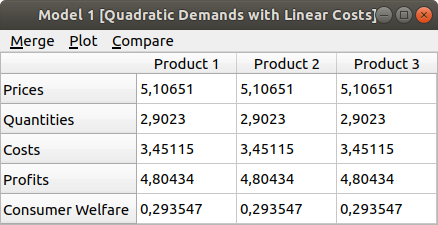
\includegraphics[width=10 cm]{first_results}
\caption{\label{first_results} Output after Loading Data}
\end{center}
\end{figure}

\begin{table}
\begin{center}
\begin{minipage}{1in}
\begin{tabular}{c}
a\\
\hline
\hline
3\\
\hline
30\\
30\\
30\\
\end{tabular}
\end{minipage}
\begin{minipage}{1in}
\begin{tabular}{c}
v\\
\hline
\hline
3\\
\hline
2\\
2\\
2\\
\end{tabular}
\end{minipage}
\begin{minipage}{1in}
\begin{tabular}{c}
w\\
\hline
\hline
3\\
\hline
0.5\\
0.5\\
0.5\\
\end{tabular}
\end{minipage}
\begin{minipage}{1.5in}
\begin{tabular}{ccc}
&B&\\
\hline
\hline
3&3&\\
\hline
-4&1.9&1.9\\
1.9&-4&1.9\\
1.9&1.9&-4\\
\end{tabular}
\end{minipage}
\begin{minipage}{1in}
\begin{tabular}{ccc}
&E&\\
\hline
\hline
3&3&\\
\hline
-1&0&0\\
0&-1&0\\
0&0&-1\\
\end{tabular}
\end{minipage}
\caption{\label{tab:input}Data Set Introduced to Obtain Figure \ref{first_results}}
\end{center}
\end{table}

From here users can compute a merger, by clicking on "Merge". In figure \ref{merge_1}, we see the initial interface the user is faced with. By clicking "Add group", the user can create a separate list of firms that would merge. It is possible to create several groups, and if every group contains only one product the market remains the same. As we see in figure \ref{merge_2}, the user may add products by selecting them on the left and clicking "Add". Similarly, be selecting products on the right and clicking "Remove" they can do exactly that. Once the new market concentration is determined, the user should click "Apply".
\begin{figure}
\begin{center}
\begin{minipage}{2.75in}
  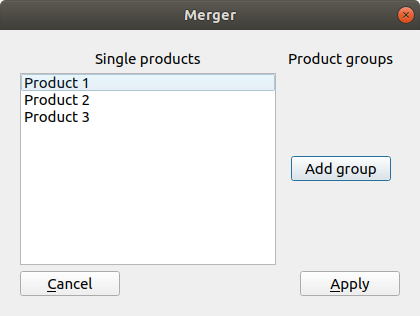
\includegraphics[width=5 cm]{merge_1}
\caption{\label{merge_1} Initial Interface of the Merge Function}
\end{minipage}
\begin{minipage}{2.75in}
 
\includegraphics[width=5 cm]{merge_2}
\caption{\label{merge_2} Interface to Create Merging Groups}
\end{minipage}
\end{center}
\end{figure}

In figure \ref{after_merger}, we see the new market equilibrium values after the merger. Note that this one is called "Model 2", since the parameters are not the same as in the previous phase. From this point, it is interesting to be able to compare the two models, which we can do by clicking on "Compare".
\begin{figure}[H]
\begin{center}
  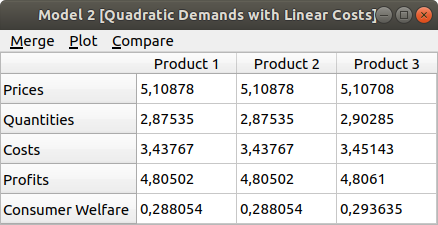
\includegraphics[width=10 cm]{after_merger}
\caption{\label{after_merger} New Market Equilibrium after Merger}
\end{center}
\end{figure}

The function "Compare" returns the difference between pre and post-merger values. As we can see in figure \ref{compare}, prices and profits have increased after the merger, while quantities, costs and consumer welfare have dropped. Thus, the compare function highlights the variation, allowing the user to better comprehend the consequences of the merger. 
\begin{figure}[H]
\begin{center}
  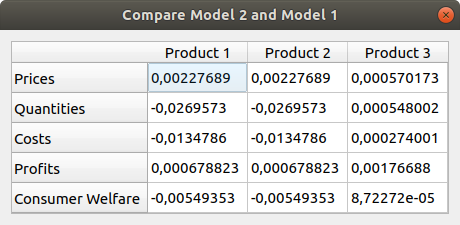
\includegraphics[width=10 cm]{compare}
\caption{\label{compare} Output of the Compare Function for Model 1 and Model 2}
\end{center}
\end{figure}

Going back to figure \ref{after_merger}, we see that there is also de function "Plot".
\begin{figure}
\begin{center}
\begin{minipage}{2.75in}
  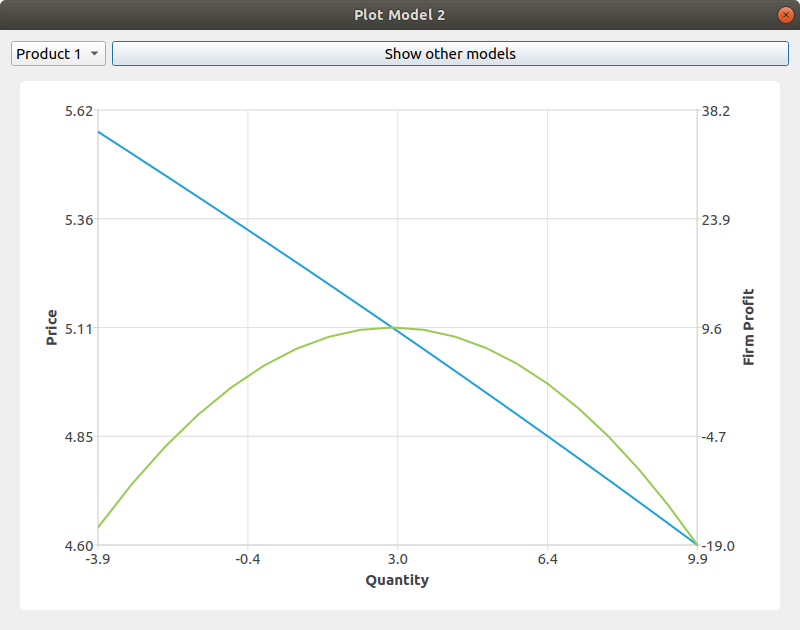
\includegraphics[width=5 cm]{plot_1}
\caption{\label{plot_1} Plot for Model 2}
\end{minipage}
\begin{minipage}{2.75in}
 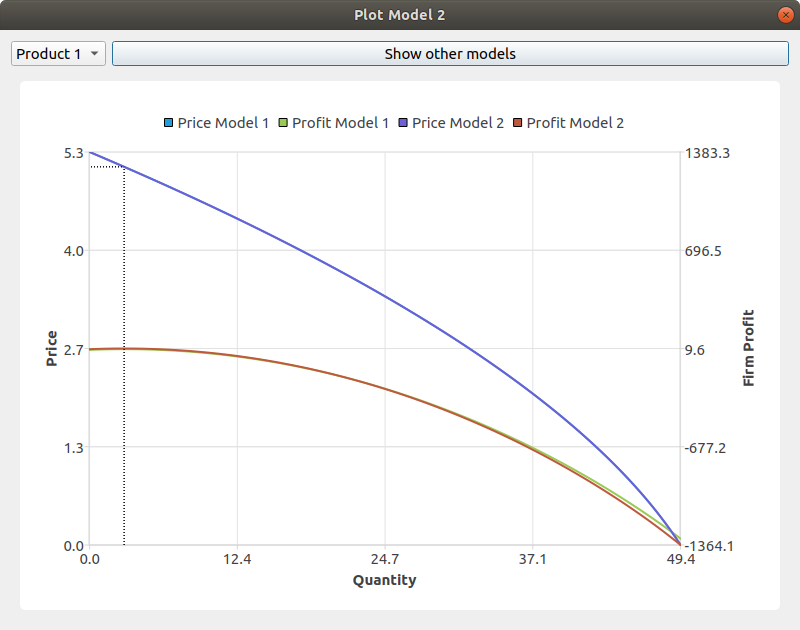
\includegraphics[width=5 cm]{plot_2}
\caption{\label{plot_2} Plot for Model 1 and Model 2}
\end{minipage}
\end{center}
\end{figure}

\section{Conclusion}

\newpage
\begin{thebibliography}{9}

\bibitem{peters}
Peters, C. (2006). Evaluating the performance of merger simulation: Evidence from the US airline industry. The Journal of law and economics, 49(2), 627-649.

\bibitem{ivaldi}
Ivaldi, M., \& Verboven, F. (2005). Quantifying the effects from horizontal mergers in European competition policy. International Journal of Industrial Organization, 23(9-10), 669-691.

\bibitem{bjorn}
Bj\"{o}rnerstedt, J., \& Verboven, F. (2016). Does merger simulation work? Evidence from the Swedish analgesics market. American Economic Journal: Applied Economics, 8(3), 125-64.

\bibitem{davis}
Davis, P. (2006). Coordinated effects merger simulation with linear demands.
\end{thebibliography}


\newpage
\listoffigures

\newpage
\listoftables

\newpage
\section*{Appendix 1: Computation of the Integral of the Consumer Welfare for Quadratic Models}

Write the demand function as follows,
\begin{equation} \label{demand}
q_k = a_k + \sum_{j \neq k} b_{jk} \cdot p_j + \sum_{j \neq k} e_{jk} \cdot p_j^2 + b_{kk} \cdot p_k + e_{kk} \cdot p_k^2
\end{equation}

Now, consider the following,
\begin{equation} \label{H}
H = a_k + \sum_{j \neq k} b_{jk} \cdot p_j + \sum_{j \neq k} e_{jk} \cdot p_j^2
\end{equation}

Combining \ref{demand} and \ref{H}, and equalizing to $0$ we obtain,
\begin{equation*}
0 = H + b_{kk} \cdot p_k + e_{kk} \cdot p_{kk}^2
\end{equation*}

This follows the structure of a second degree equation, which can be easily solved. Then, consider the following,
\begin{equation*}
\Delta = b_{kk}^2 - 4 \cdot e_{kk} (H - q_k) = b_{kk}^2 - 4 \cdot e_{kk} \cdot H + 4 \cdot e_{kk} \cdot q_k 
\end{equation*}

Therefore, we obtain,
\begin{equation*}
p_k = \frac{-b_{kk}}{2 \cdot e_{kk}} \pm \frac{\sqrt{\Delta}}{2 \cdot e_{kk}}
\end{equation*}

Let us now decide on the sign. Inside $\sqrt{\Delta}$, the factor multiplying $q_k$ is negative, since $e_kk < 0$. Looking at the plots of $y = \sqrt{-x}$ and $y = -\sqrt{-x}$, we can make such an assessment.\\

\begin{figure}[H]
    \begin{minipage}{0.45\textwidth}
\begin{tikzpicture}
\begin{axis}[
  axis lines=middle,
  clip=false,
  ymin=0,
  xticklabels=\empty,
  yticklabels=\empty,
  legend pos=north west
]
\addplot+[mark=none,samples=200,unbounded coords=jump] {sqrt(-x)};
\legend{$y=\sqrt{-x}$}
\end{axis}
\end{tikzpicture}        
\caption{$y = \sqrt{-x}$}
\end{minipage}\hfill
\begin{minipage}{0.45\textwidth}
\begin{tikzpicture} 
\begin{axis}[
  axis lines=middle,
  clip=false,
  ymin=-3,
  xticklabels=\empty,
  yticklabels=\empty,
  legend pos=north west
]
\addplot+[mark=none,samples=200,unbounded coords=jump] {-sqrt(-x)};
\legend{$y=-\sqrt{-x}$}
\end{axis}
\end{tikzpicture}       
\caption{$y = -\sqrt{-x}$}
    \end{minipage}
\end{figure}

From here, it is clear that the demand function should look like the first one. Since we divide by $2 \cdot e_{kk} <0$, we choose the negative root. Hence,
\begin{equation*}
p_k(q_k) = \frac{-b_{kk}}{2 \cdot e_{kk}} - \frac{\sqrt{\Delta}}{2 \cdot e_{kk}}
\end{equation*}

With this approach, it is easier to compute the are comprised by the producers' revenue and consumer surplus, and then substract the former. Thus, we first want to compute
\begin{equation} \label{integral}
\int_0^{q_k^*} p_k(q_k) \ dq_k = -\frac{b_{kk}}{2 \cdot e_{kk}} \cdot q^* -\frac{1}{2 \cdot e_{kk}} \cdot \bigg[\frac{2}{12 \cdot e_{kk}} (b_{kk}^2 - 4 \cdot e_{kk}(H - q))^{\frac{3}{2}}\bigg]_0^{q^*}
\end{equation}

Finally to obtain the consumer surplus as a measure of consumer welfare, we substract revenue from equation \ref{integral}, such that,
\begin{equation}
CW_k= \int_0^{q_k^*} p_k(q_k) \ dq_k  - p_k^* \cdot q_k^*
\end{equation}

%
\end{document}
%--------------------------------------------------------------%
%--------------------------------------------------------------%
